\likechapter{Постановка задачи и исходные данные}

\textbf{Цель работы} 

Управление манипуляционным роботом \textit{KUKA youBot} на основе решения обратной задачи о положениях при перемещении схвата по заданному закону.

\textbf{Ограничения}

В лабораторных рассматривается только две степени манипулятора -- остальные зафиксированы. Из этого следует, что: $ \phi_1, \phi_4 $ и $ \phi_5 $ это константы, а угол ориентации схвата в плоскости руки манипулятора: $\theta = \phi_2+\phi_3+\phi_4$. Причем, последнее звено схвата выпрямлено, находится в положении параллельном третьему звену, откуда следует, что $ \phi_4=0 $.

\textbf{Исходные данные}

\begin{figure}[ht!]
    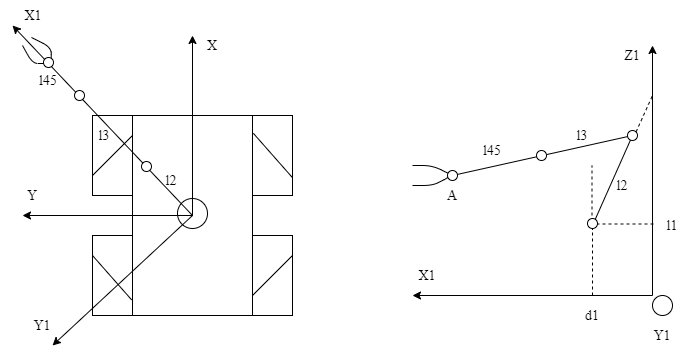
\includegraphics[width=1.0\textwidth]{chapter_intro/figure1.png}
\end{figure}

Длины звеньев и расстояния между их осями:
\begin{align*}
    d_1 &= 0.033 \\
    l_1 &= 0.075 \\
    l_2 &= 0.155 \\
    l_3 &= 0.135 \\
    l_4 &= 0.081 \\
    l_5 &= 0.137 \\
    l_{45} &= l_4+l_5 = 0.218 \\
    l_{345} &= l_3 + l_4 + l_5 = 0.353
\end{align*}

Схват перемещается так, что его координаты $X$ и $Y$ не меняются со временем, а $Z$ меняется по закону:
$$ Z(t) = 0.2 + 0.1 \cos \frac{2 \pi t}{10} $$

Время берем дискретное, из ста значений от $0$ до $10 \: c$. Временной шаг $ \Delta t = 0.1 \: с $

Так как для управления движением манипулятора используются «технические» углы $A_i$, отсчет которых производится от упоров, то необходим переход от углов $\varphi_i$ к $A_i$, который осуществляется следующим образом:
\begin{align*}
    A_1 &= \varphi_1+2.9496 \\
    A_2 &= \varphi_2+1.1345 \\
    A_3 &= \varphi_3-2.5654 \\
    A_4 &= \varphi_4+1.829 \\
    A_5 &= -\varphi_5+2.93 
\end{align*}

Причем диапазоны работы манипулятора ограничены в $A_i$:
\begin{align*}
   0.01 &< A_1 < 5.84 \\
   0.01 &< A_2 < 2.6179 \\
   -4.8 &< A_3 < -0.01 \\
   0.022 &< A_4 < 3.4292 \\
   0.01 &< A_5 < 5.6415 
\end{align*}

Нам заданы $X(t)$,$Z(t)$, требуется найти $\varphi_i (t)$.